\documentclass[a4paper]{article}
\usepackage{geometry}
\geometry{a4paper, portrait, margin=1in}
\usepackage[english]{babel}
\usepackage[utf8]{inputenc}
\usepackage{natbib}
\usepackage{graphicx}
\usepackage{fancyhdr}
\usepackage{array}
\usepackage{tabu}
\usepackage{listings}
\usepackage[export]{adjustbox}
\graphicspath{{/Users/ThomasBass/GitHub/GSCE-Coursework-Weblang-Q3-TrafficLights/Images/}}
%%\DeclareGraphicsExtensions{.png}


\title{Computing GCSE Coursework}
\author{\\ \\ \\ \\ Thomas Bass\\Candidate 4869\\Centre 52423\\OCR A452 Practical Investication\\\\Made with \LaTeX}
\date{2017}


\pagestyle{fancy}
\fancyhf{}
\rhead{Computing GCSE Coursework}
\chead{Candidate 4869}
\lhead{Thomas Bass}
\rfoot{Page \thepage}

\begin{document}

\maketitle
\pagebreak
\renewcommand*\contentsname{Summary}
\tableofcontents
\pagebreak

%%%%%%%%%%%%%%%%%%%%%%%%%%%%%%%%%%%%%%%%%%%%%%%%%%%%%%%%%%%%%%%%%%%%%%%%%

\section{Task 1}
Often, a web designer wants a change to happen when a user clicks on a screen object or moves the mouse over it. JavaScript can make changes to the HTML elements. \par
\noindent Enter and run this script: \par \par
\begin{lstlisting}
<!DOCTYPE html>
<html>
<body>
<h1>Change an HTML element</h1>
<p id="msg">Now you see me.</p>
<button type="button"
onclick="document.getElementById('msg').innerHTML = 'Gone!'">
Click Me!</button>
<button type="button"
onclick="document.getElementById('msg').innerHTML = 'Back again!'">
Bring me back!</button>
</body>
</html>
\end{lstlisting}
	

\subsection{Explain how you ran this script:} ~\par	

This script was copied into a HTML document, and opened into a web browser. 

When the script ran it gave the following output: ~\par ~\par
\noindent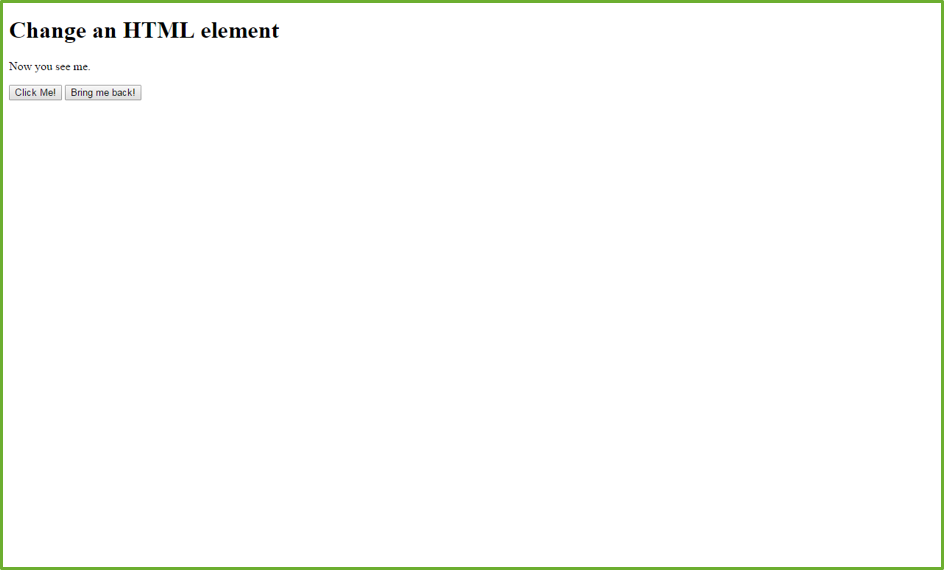
\includegraphics[width=0.5\textwidth, left, width=\linewidth, frame]{Picture1.png} \par 

The web page took the code entered, ran it, and produced this output.
\newpage
\subsection{Explain what each line of the script does:}
\subsubsection{The HTML Code:}
\begin{lstlisting}
01	<!DOCTYPE html>
02	<html>
03	<body>
04	<h1>Change an HTML element</h1>
05	<p id="msg">Now you see me.</p>
06	<button type="button"
07	onclick="document.getElementById('msg').innerHTML = 'Gone!'">
08	Click Me!</button>
09	<button type="button"
10	onclick="document.getElementById('msg').innerHTML = 'Back again!'">
11	Bring me back!</button>
12	</body>
13	</html>
\end{lstlisting}
\subsubsection{Commentry:}

\begin{lstlisting}
01	This declares that the document is a HTML document
02	This opens the <html> tag, and shows that the code enclosed 
	is HTML code
03	This opens the <body> tag, and shows that the code enclosed 
	is placed in the body of the document
04	This opens the <h1> tag, showing that the text enclosed 
	("Change an HTML Element") is placed in the highest header, and closes
	the tag
05	This opens a <p> tag, showing that the text enclosed ("Now you see me.")
	is paragraph text, and it has the ID "msg", and then the tag is closed
06	This opens a <button> tag, showing that the information enclosed is 
	a button, and has type "button"
07	This declares that following an onclick event (when the button is clicked),
	the program will execute a Javascript function to find the elements with 
	the ID of "msg" (the body text in line 05) and change its HTML code to "Gone".
08	This line provides the text of the button ("Click Me!") and closes the 
	<button> tag
09	This opens a <button> tag, showing that the information enclosed is 
	a button, and has type "button"
10	This declares that following an onclick event (when the button is clicked),
	the program will execute a Javascript function to find the elements with 
	the ID of "msg" (the body text in line 05) and change its 
	HTML code to "Back Again!".
11	This line provides the text of the button ("Bring me back!") and closes the 
	<button> tag
12	This closes the <body> tag
13	This closes the <body> tag and ends the document
\end{lstlisting}
\newpage
%%%%%%%%%%%%%%%%%%%%%%%%%%%%%%%%%%%%%%%%%%%%%%%%%%%%%%%%%%%%%%%%%%%%%%%%%
\section{Task 2}
As is the case with most programming languages, in JavaScript you can use arrays in order to store multiple values under the same identifier. For example, an array of products can be set up as below for use on an ecommerce web site.\par
  \verb|var products = ["Printer","Tablet","Router"];|

\subsection{Set up an array to include the items shown above, plus a few extras of your choice.}








\end{document}